\def \bkgestimationPlotsDir {plots/bkgestimation/}

\section{Background Estimation Method}
\label{sec:bkgest}


%Note, this is equivalent to saying that the ratio of yeilds in the
%tagged region and the yields in the anti-tagged region, R$_{pass/fail}$, is independent of the mass. 
%\begin{figure}[htbp!]

%  \begin{center}
%    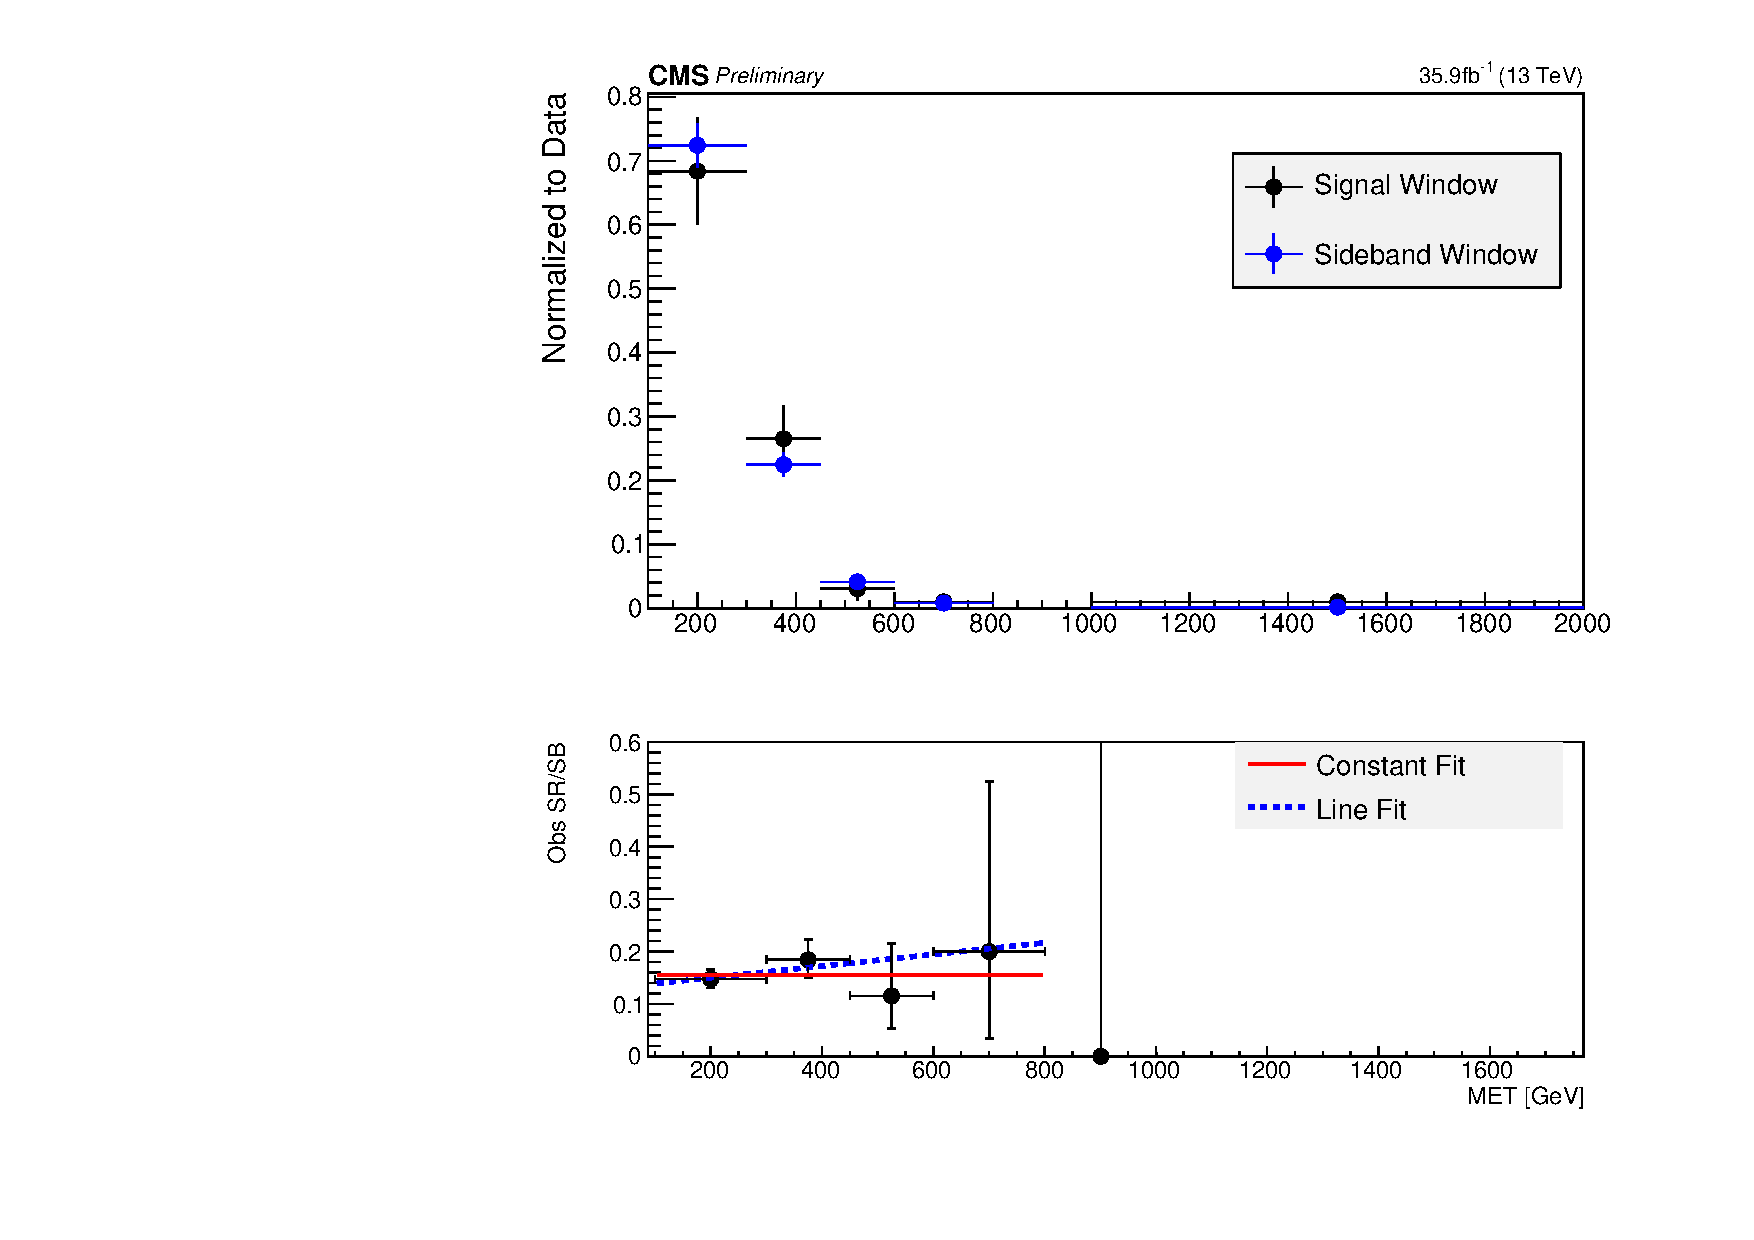
\includegraphics[trim={5px 5px 5px 5px},clip,width=0.6\linewidth]{plots/bkgestimation/Data2016SingleLepton.pdf}
%    \caption{ 2016 Data validation of SR and SB 
%    }
%    \label{fig:Data2016SingleLepton}
%  \end{center}
%\end{figure} 


\begin{figure}[htbp!]
  \begin{center}
    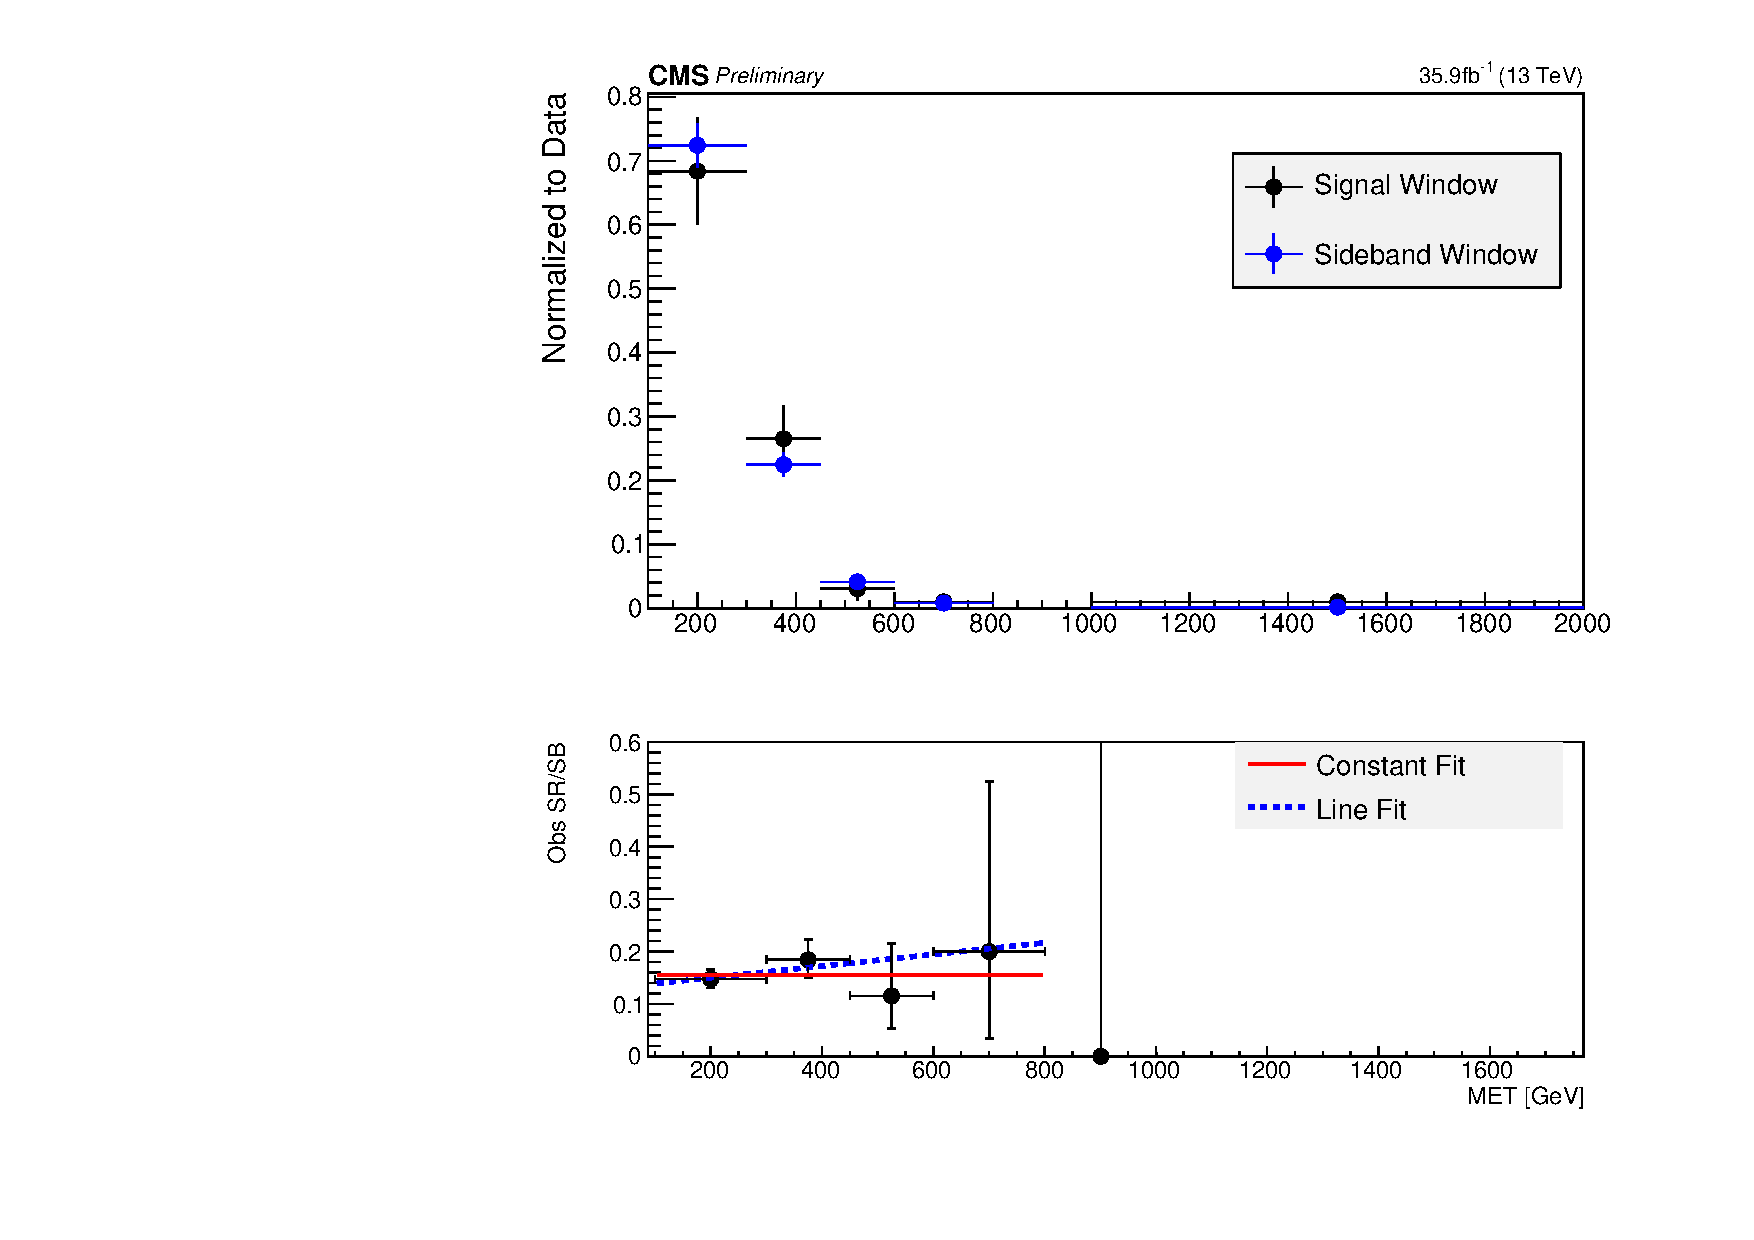
\includegraphics[trim={5px 5px 5px 5px},clip,width=0.48\linewidth]{plots/bkgestimation/Data2016SingleLepton.pdf}\\
    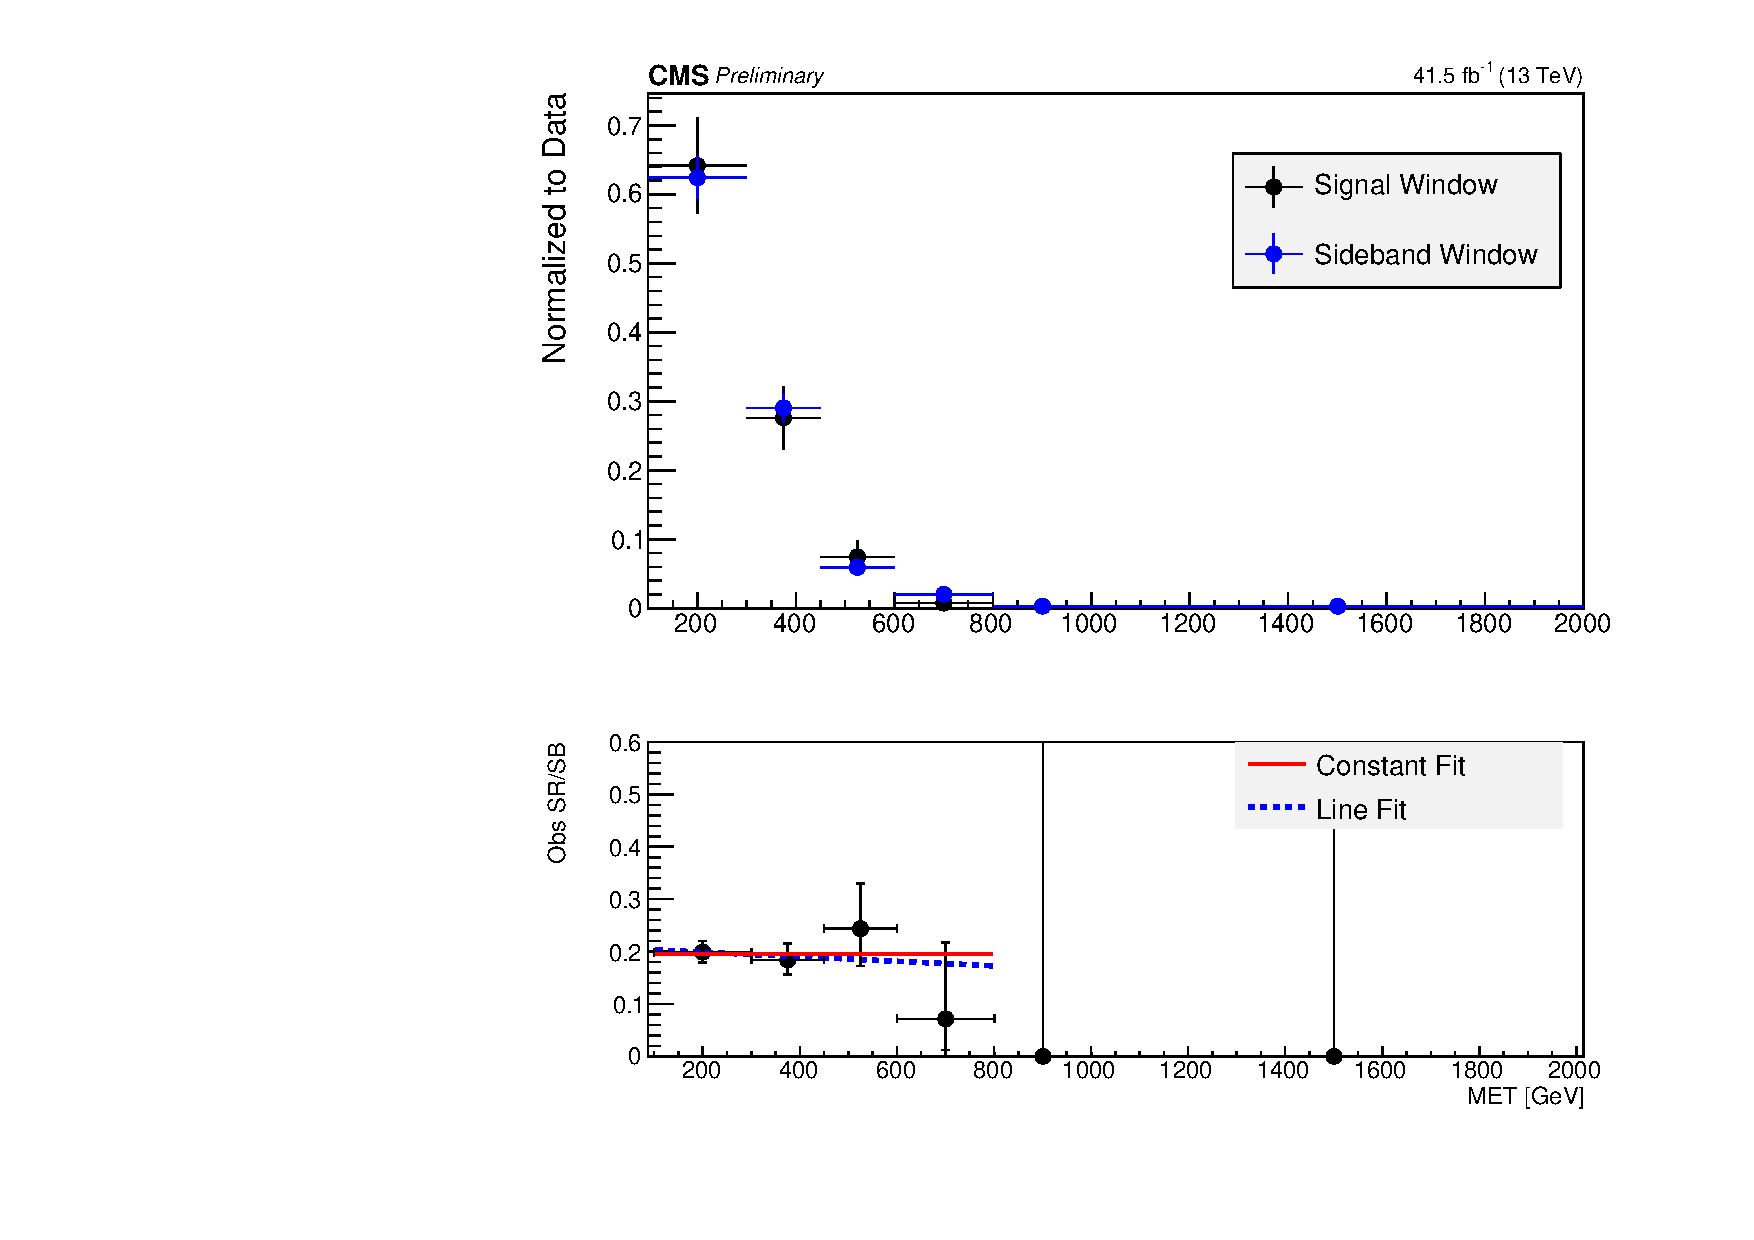
\includegraphics[trim={5px 5px 5px 5px},clip,width=0.48\linewidth]{plots/bkgestimation/Data2017SingleLepton.pdf}
    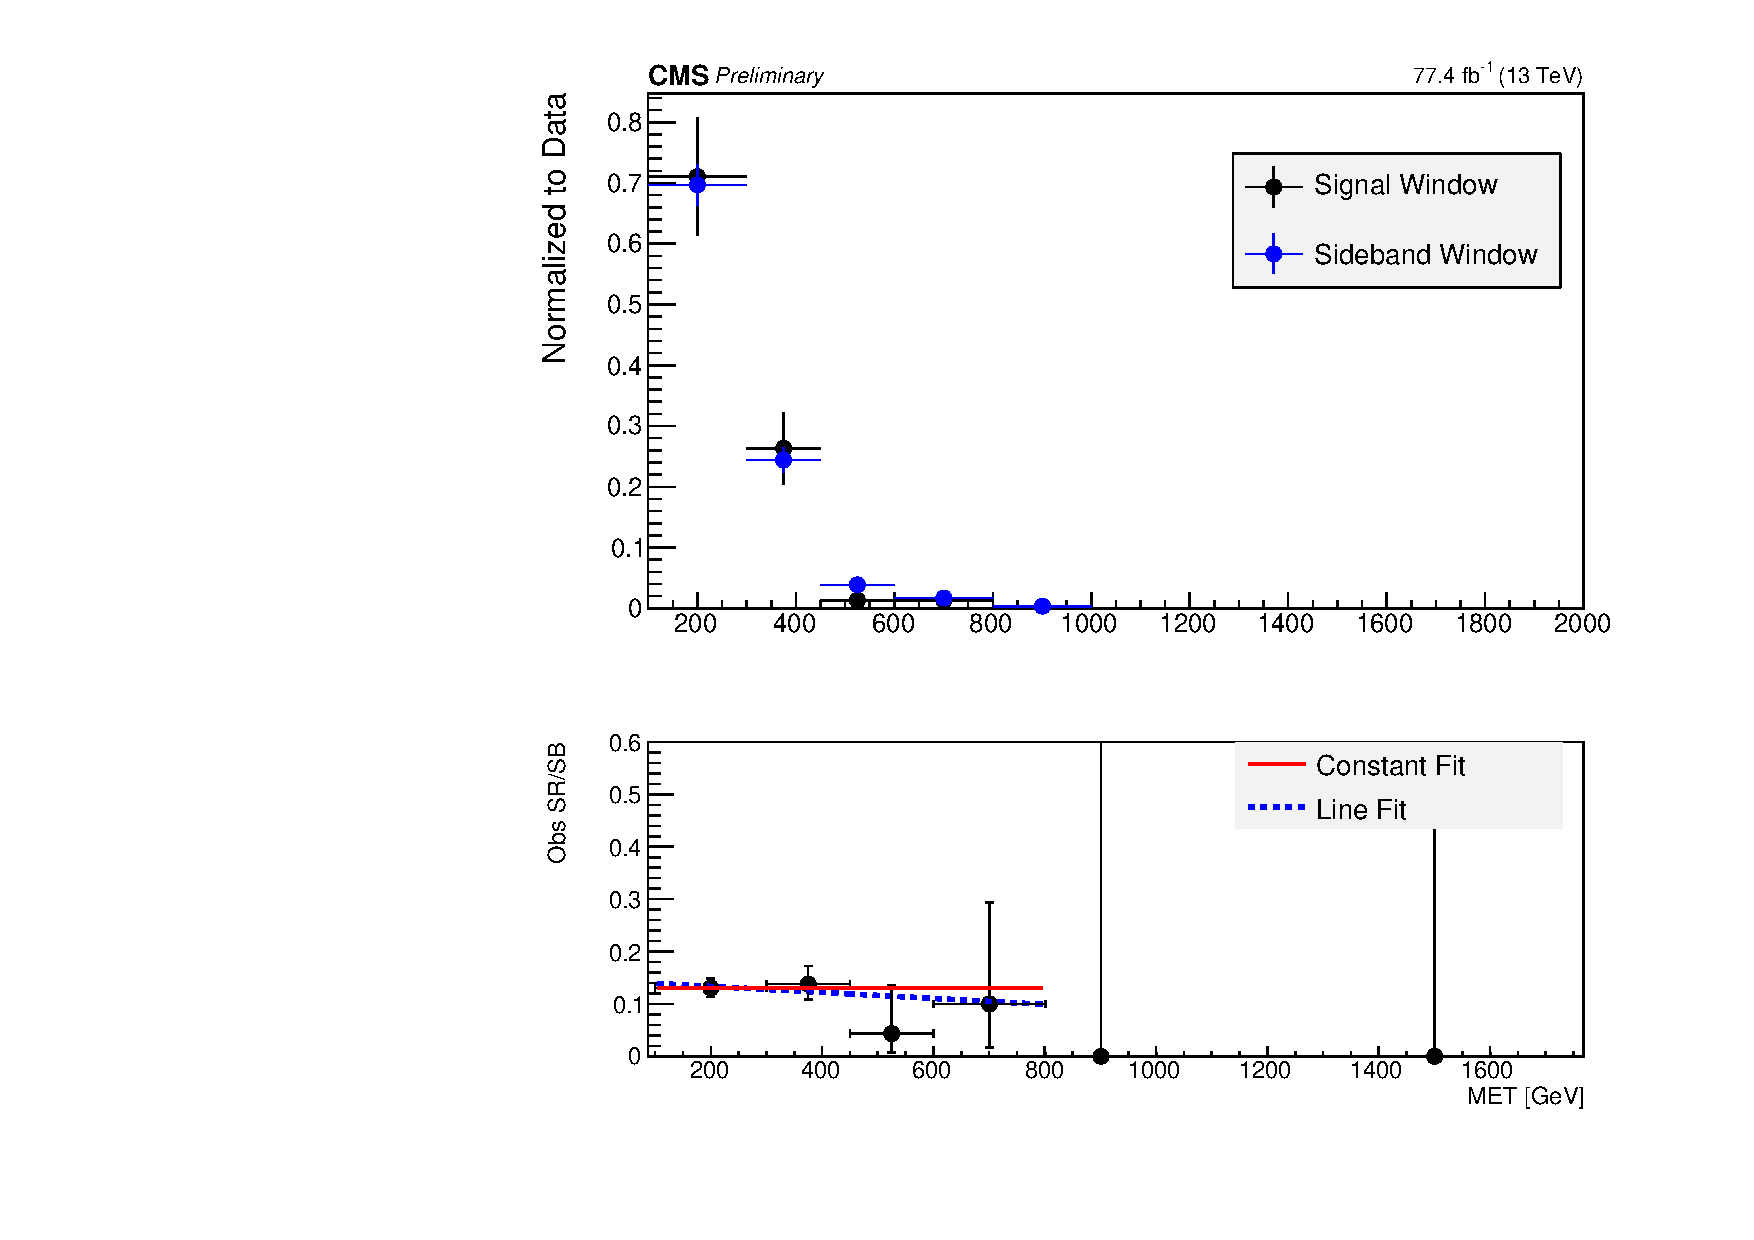
\includegraphics[trim={5px 5px 5px 5px},clip,width=0.48\linewidth]{plots/bkgestimation/Data2018SingleLepton.pdf}
    \caption{single photon validation region from 3 eras of 2016(left), 2017(middle) and 2018(right)}
    \label{fig:DataSingleLepton}
  \end{center}
\end{figure} 

\begin{figure}[htbp!]
  \begin{center}
    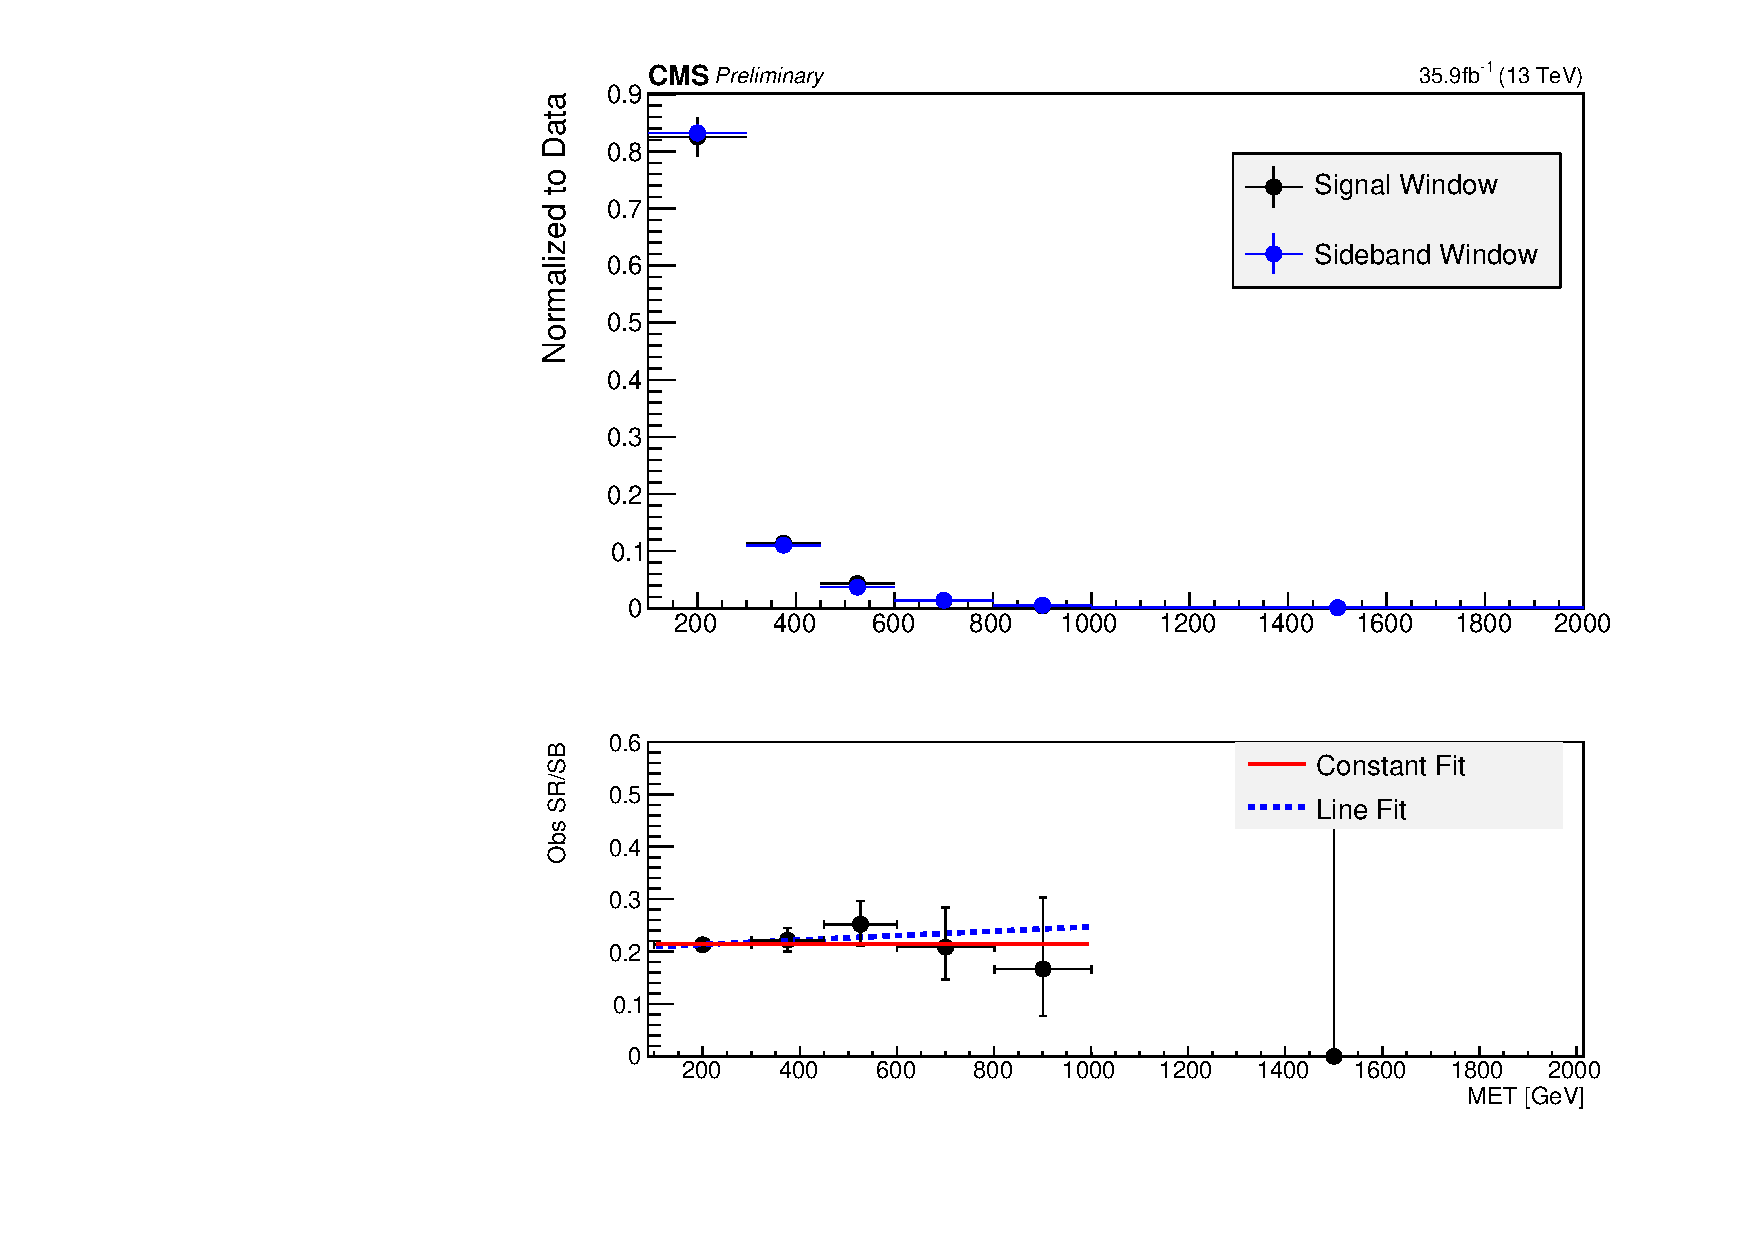
\includegraphics[trim={5px 5px 5px 5px},clip,width=0.48\linewidth]{plots/bkgestimation/Data2016SinglePhoton.pdf}\\
    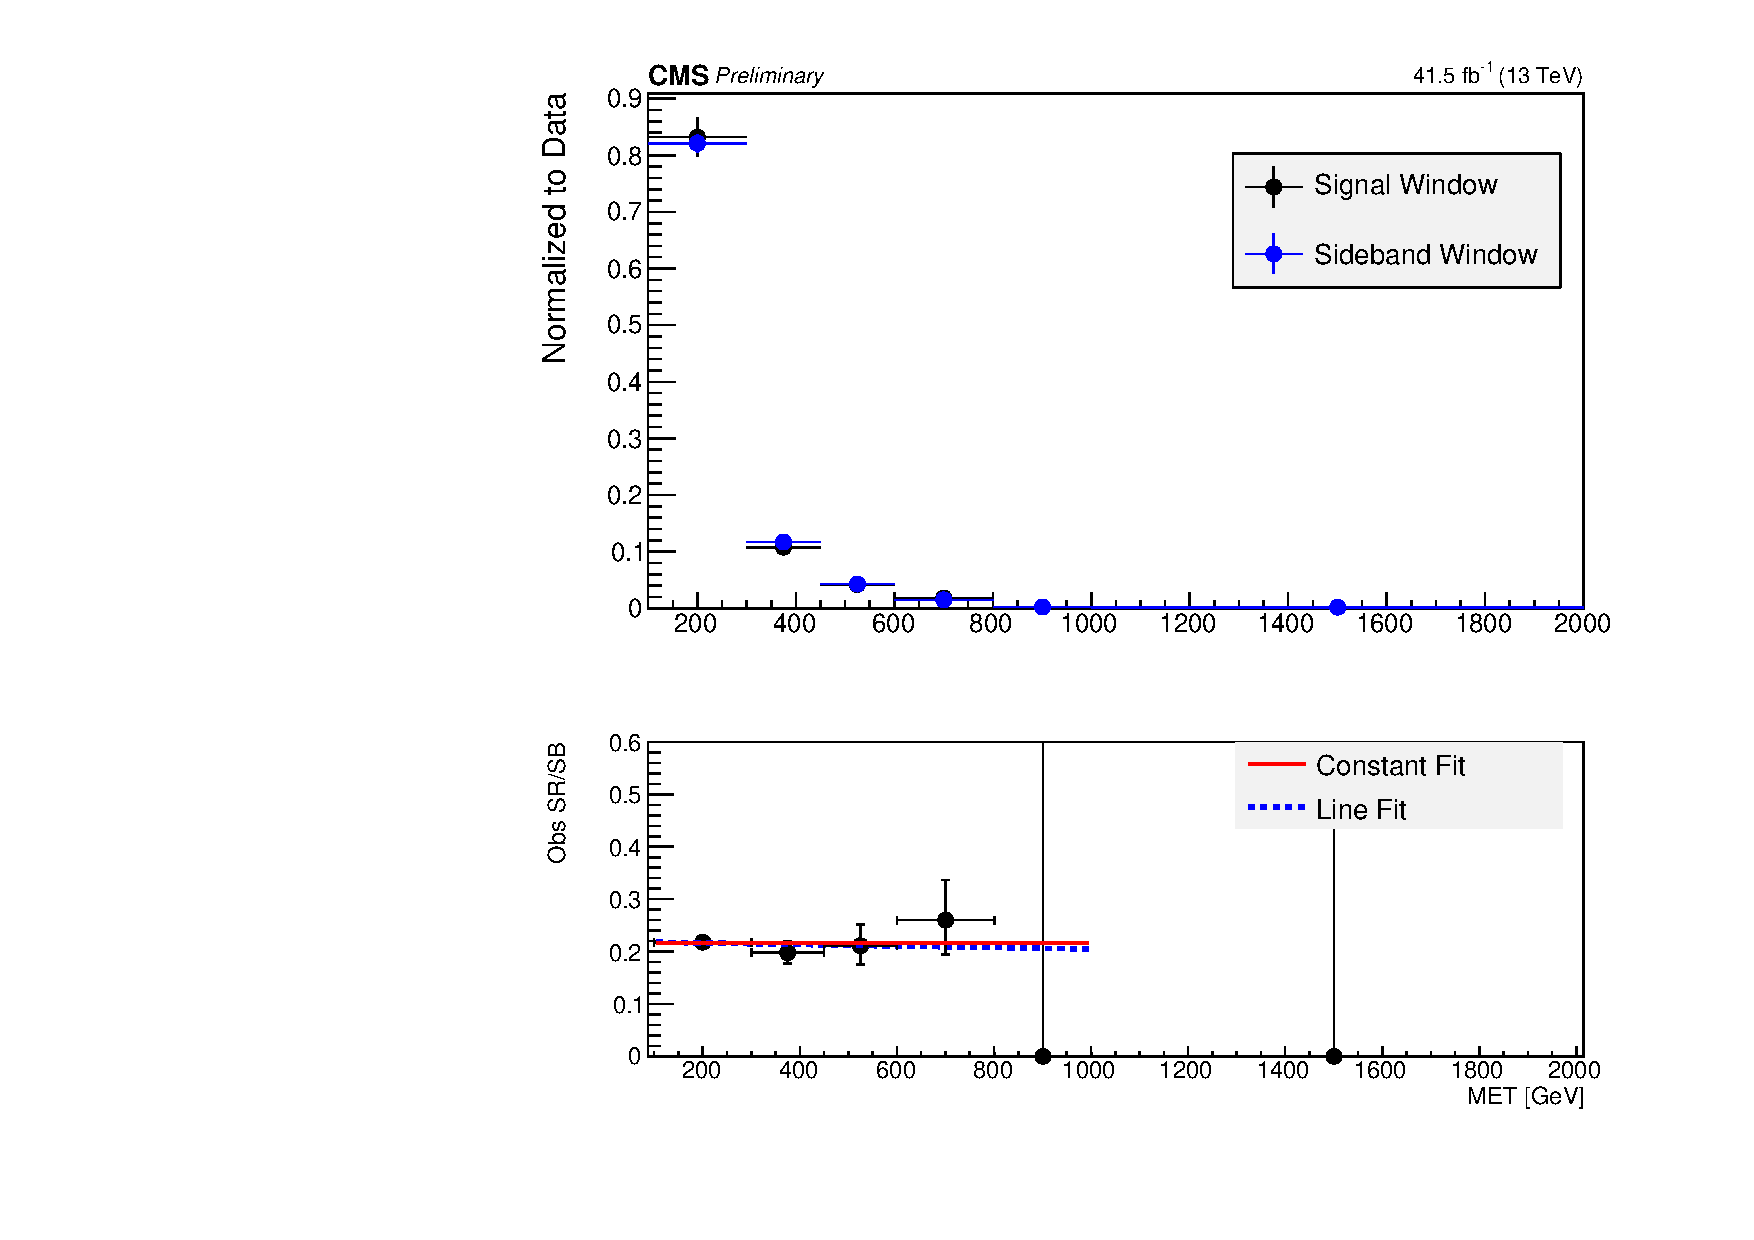
\includegraphics[trim={5px 5px 5px 5px},clip,width=0.48\linewidth]{plots/bkgestimation/Data2017SinglePhoton.pdf}
    %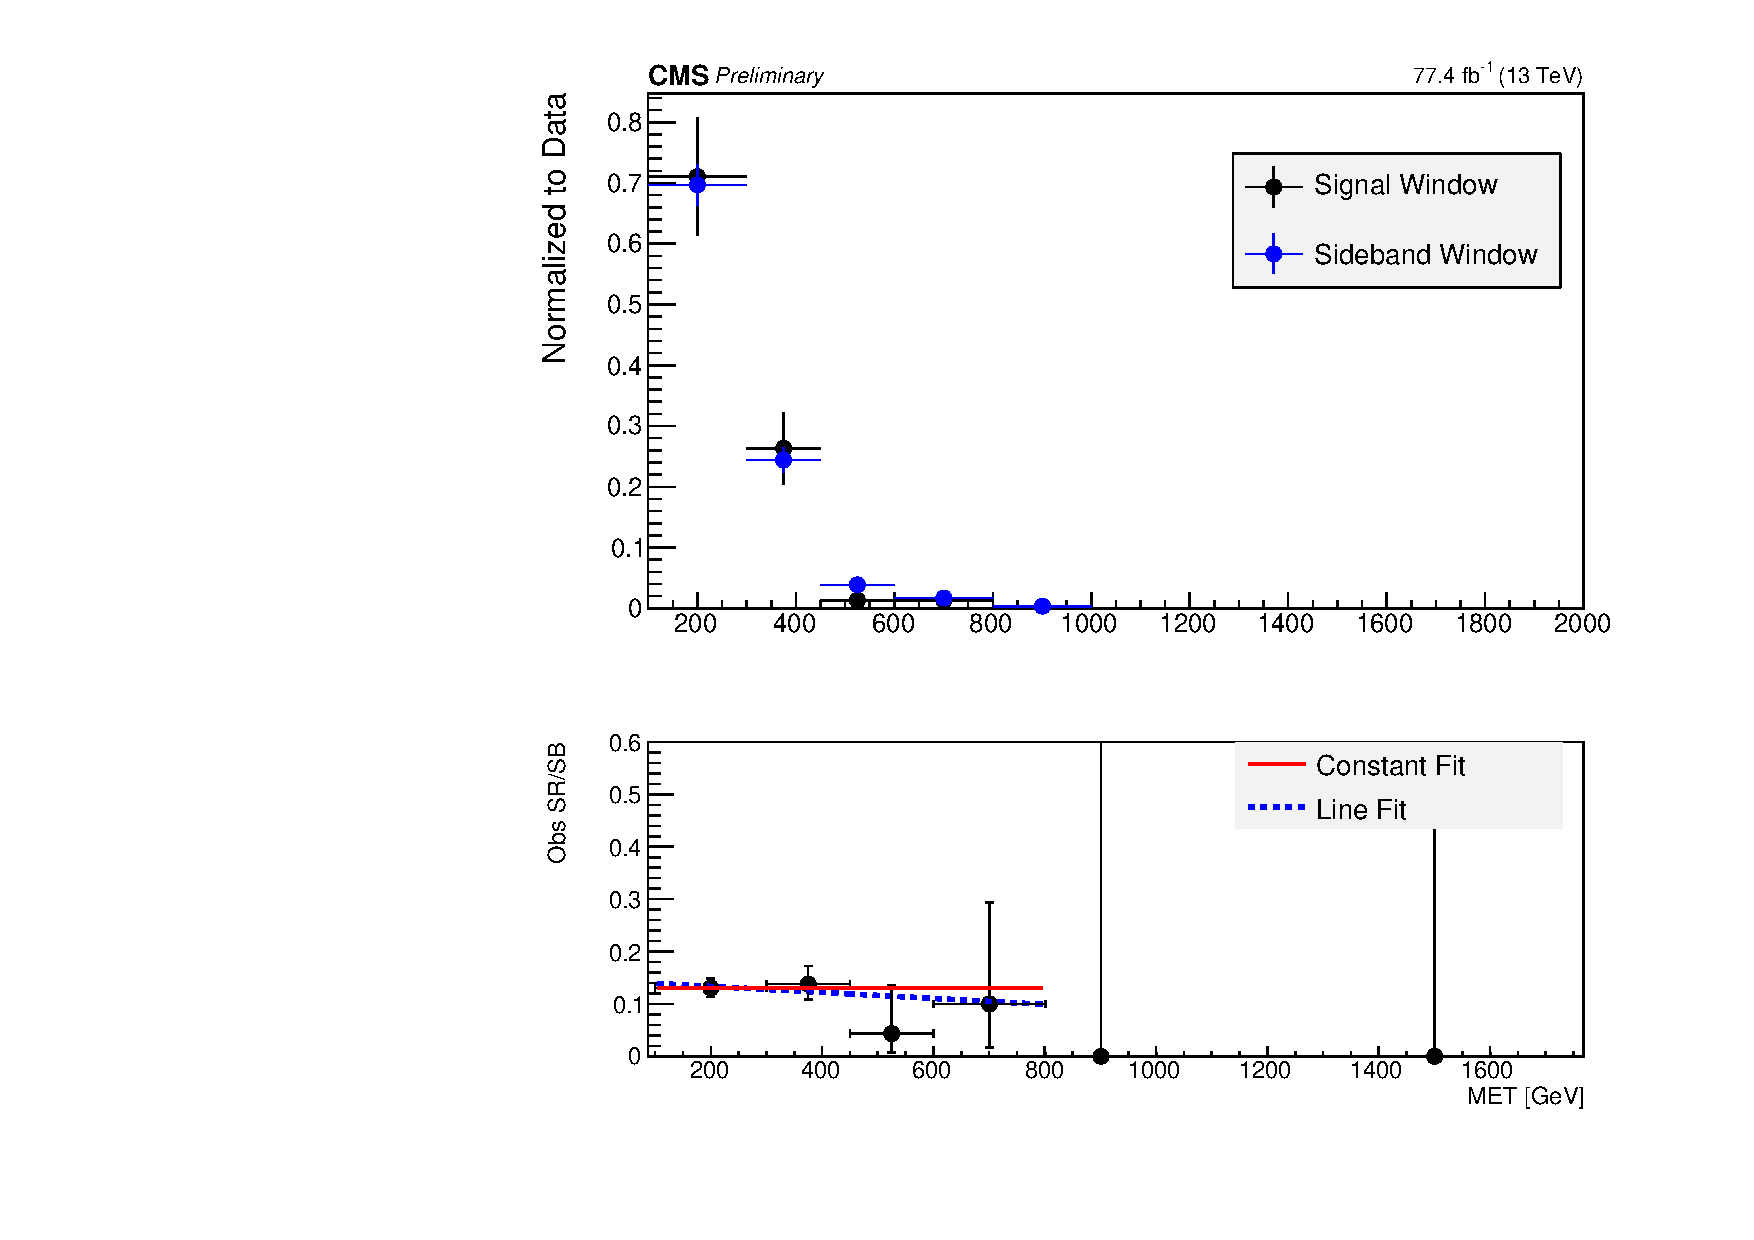
\includegraphics[trim={5px 5px 5px 5px},clip,width=0.48\linewidth]{plots/bkgestimation/Data2018SingleLepton.pdf}
    \caption{single photon validation region from 2 eras of 2016 (left) and 2017 (right)}
    \label{fig:DataSinglePhoton}
  \end{center}
\end{figure} 

\begin{figure}[htbp!]
  \begin{center}
    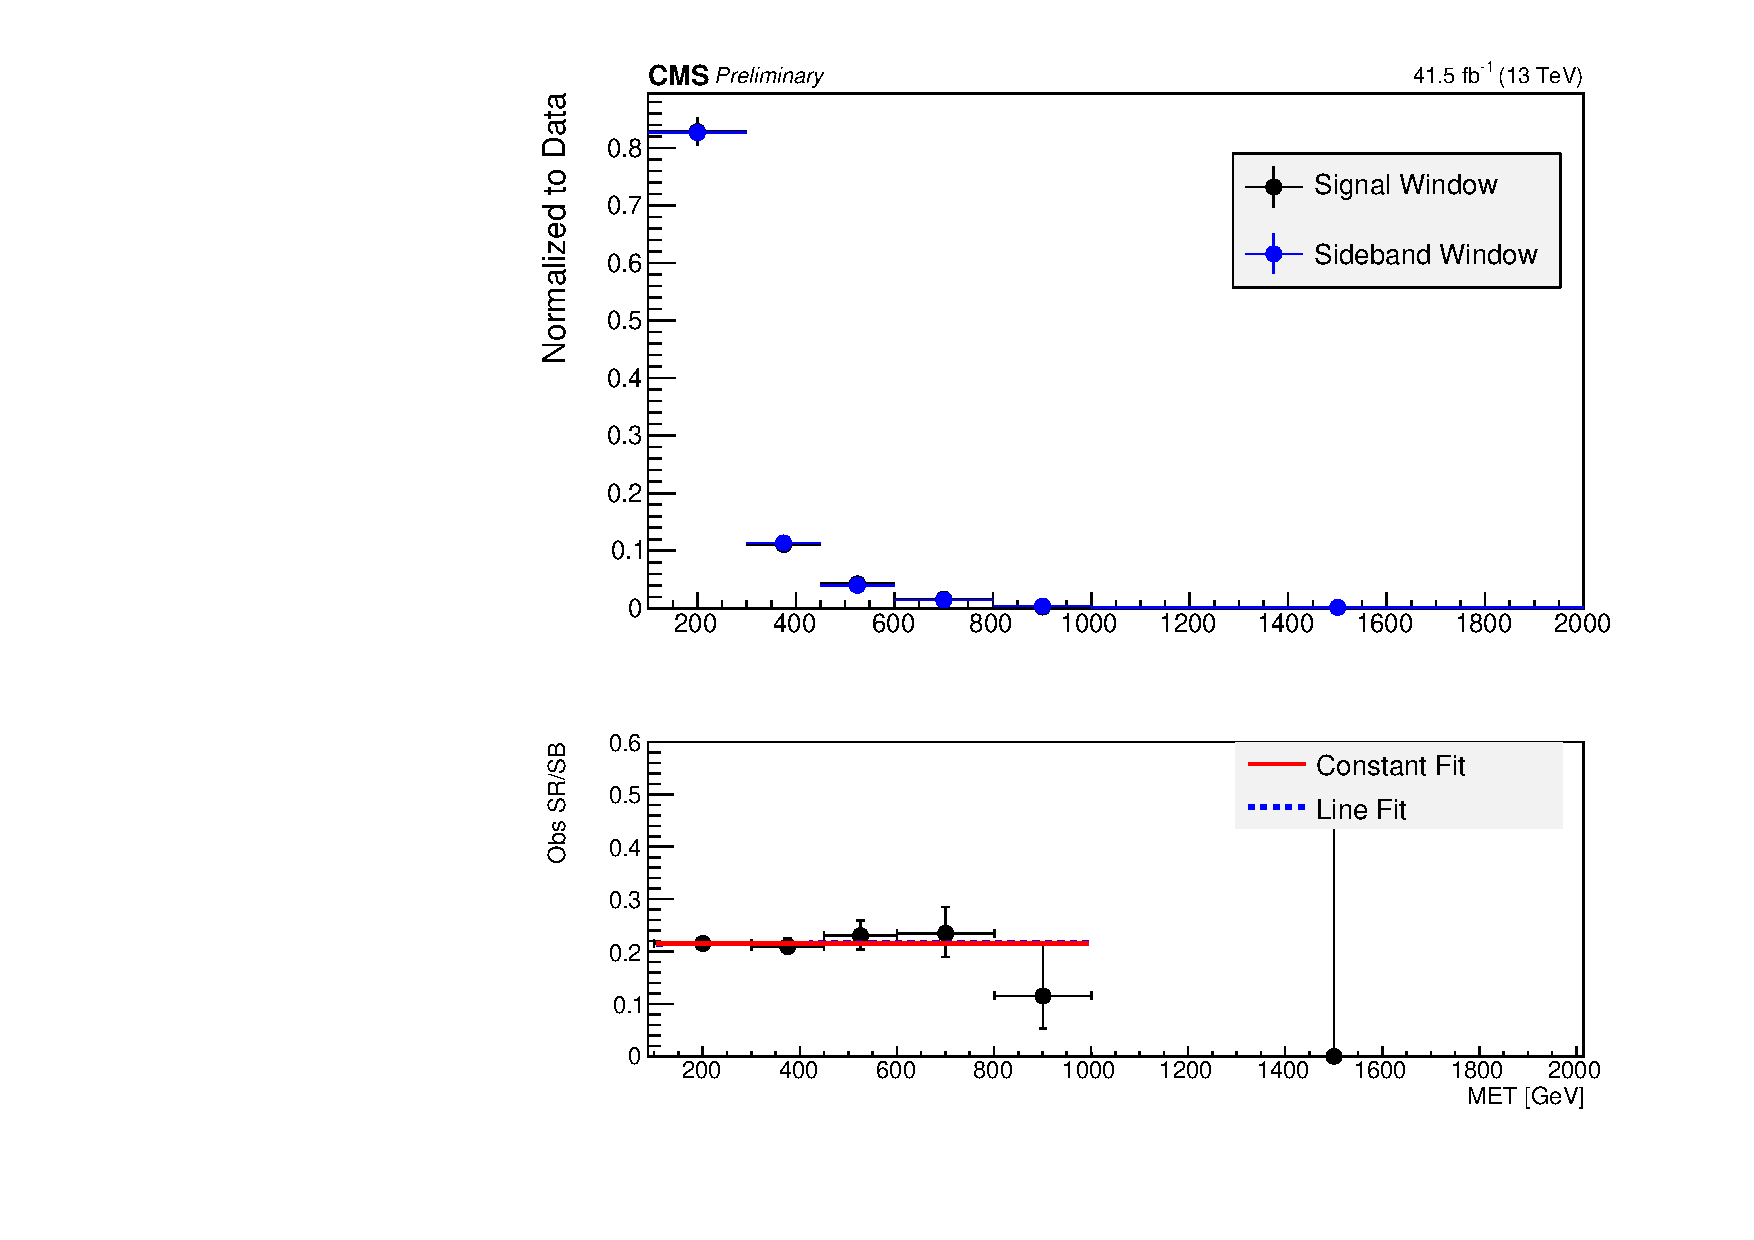
\includegraphics[trim={5px 5px 5px 5px},clip,width=0.48\linewidth]{plots/bkgestimation/DatacombinedSinglePhoton.pdf}\\
    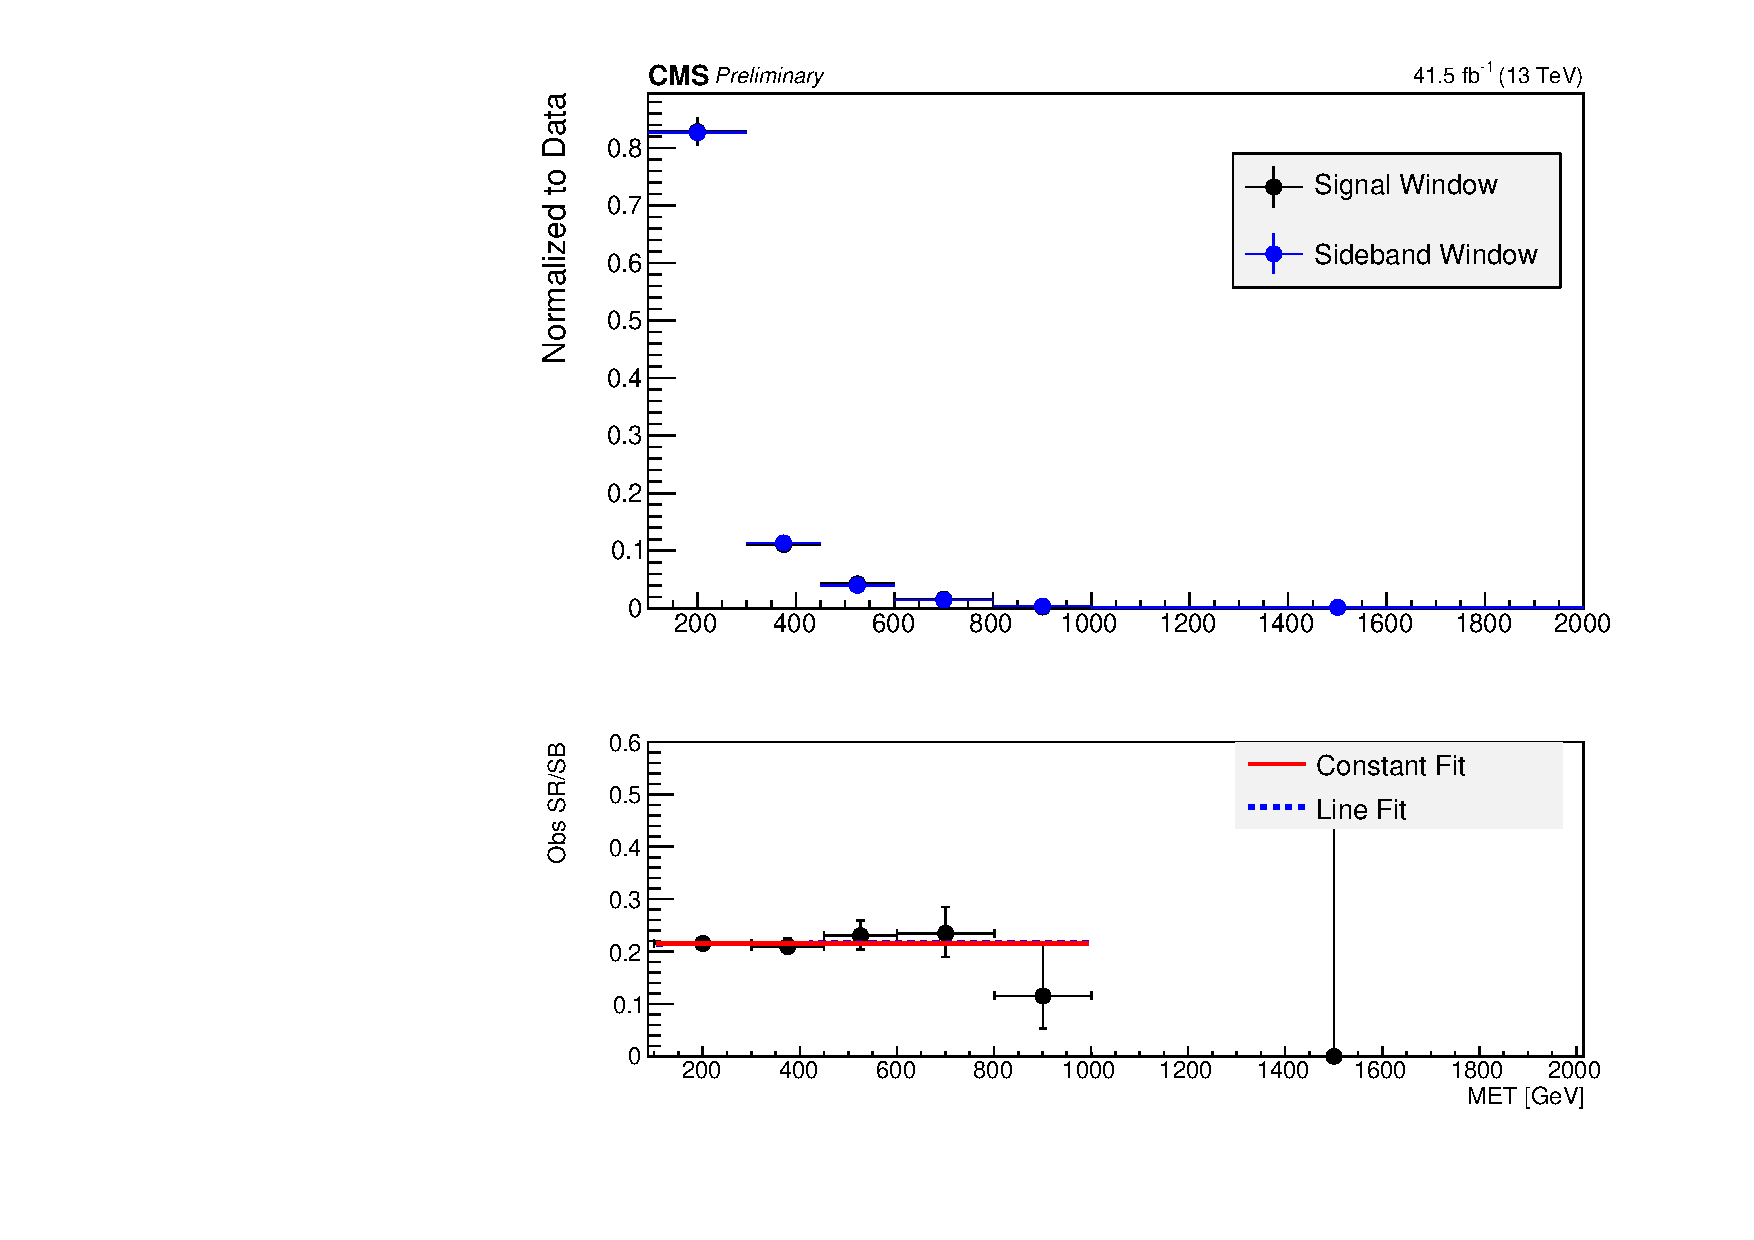
\includegraphics[trim={5px 5px 5px 5px},clip,width=0.48\linewidth]{plots/bkgestimation/DatacombinedSinglePhoton.pdf}
    \caption{combined limit for all eras of dataset for single lepton (left) and single photon (right)}
    \label{fig:DataCombinedSingleLepton}
  \end{center}
\end{figure}

\subsection{Background Systematics}
\label{sec:bkgSystematics}
 
